\documentclass{article}
\usepackage[a4paper,scale=0.8,hcentering,bindingoffset=8mm]{geometry} % A4纸大小,缩放80%,设置奇数页右边留空多一点
\usepackage{hyperref}      % 超链接
\usepackage{listings}      % 代码块
\usepackage{courier}       % 字体
\usepackage{fontspec}      % 字体
\usepackage{fancyhdr}      % 页眉页脚相关宏包
\usepackage{lastpage}      % 引用最后一页
\usepackage{amsmath,amsthm,amsfonts,amssymb,bm} %数学
\usepackage{graphicx}      % 图片
\usepackage{subfigure}
\usepackage{enumerate}
% \usepackage{subcaption}    % 图片描述
\usepackage{longtable,booktabs} % 表格
\usepackage{dot2texi}
\usepackage{tikz}
\usepackage{multirow}
\usetikzlibrary{automata, positioning, arrows}
% \usepackage{ctex}
\lstset{                  %设置代码块
         basicstyle=\footnotesize\ttfamily,% 基本风格
         numbers=left,    % 行号
         numbersep=10pt,  % 行号间隔 
         tabsize=2,       % 缩进
         extendedchars=true, % 扩展符号?
         breaklines=true, % 自动换行
         language=C,
         frame=leftline,  % 框架左边竖线
         xleftmargin=19pt,% 竖线左边间距
         showspaces=false,% 空格字符加下划线
         showstringspaces=false,% 字符串中的空格加下划线
         showtabs=false,  % 字符串中的tab加下划线
 }
\pagestyle{fancy}         % 页眉页脚风格
\fancyhf{}                % 清空当前设置
\fancyfoot[C]{\thepage\ / \pageref{LastPage}}%页脚中间显示 当前页 / 总页数,把\label{LastPage}放在最后
\begin{document} 
    \begin{titlepage}       % 封面
        \centering
        \includegraphics[width=\textwidth]{../SUSTC_LOGO.png}
        % \vspace*{\baselineskip}
        \rule{\textwidth}{1.6pt}\vspace*{-\baselineskip}\vspace*{2pt}
        \rule{\textwidth}{0.4pt}\\[\baselineskip]
        {\LARGE COMPILIER @BY 2019\\[\baselineskip]\small for SUSTech CSE}
        \\[0.2\baselineskip]
        \rule{\textwidth}{0.4pt}\vspace*{-\baselineskip}\vspace{3.2pt}
        \rule{\textwidth}{1.6pt}\\[\baselineskip]
        \scshape
        \vspace*{\baselineskip}
        {\Large HomeWork 2\par }
        Edited by \\[\baselineskip] {汪至圆\par}
        {\Large 11610634\par }
        \vfill
        {\scshape 2019} \\{\large SHENZHEN}\par
    \end{titlepage}
    \section{Exercise 1: Design finite automata (both deterministic and nondeterministic) for each of the following regular languages:}
        \subsection{ L(a(a|b)*b) [10 points]}
            \subsubsection{NFA}
                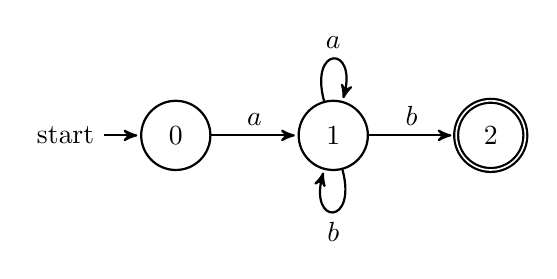
\begin{tikzpicture}[->,>=stealth',shorten >=1pt,auto,node distance=2cm,
                    thick,base node/.style={circle,draw,minimum size=16pt}, real node/.style={double,circle,draw,minimum size=35pt}]
                    \node[initial,initial text={start}, state] (1) {$0$};
                    \node[state](2)[right of=1 ]{$1$};
                    \node[state, accepting](3)[right of=2 ]{$2$};
                    \path[]
                    (1) edge node {$a$} (2)
                    (2) edge [loop above] node {$a$} (2)
                    (2) edge [loop below] node {$b$} (2)
                    (2) edge node {$b$} (3);
                \end{tikzpicture}
            \subsubsection{DFA}
            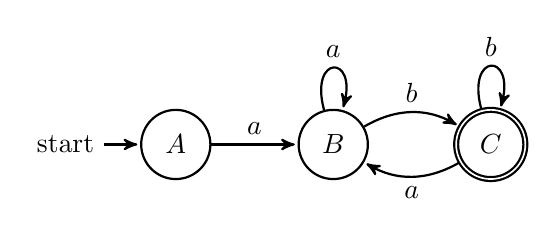
\begin{tikzpicture}[->,>=stealth',shorten >=1pt,auto,node distance=2cm,
                thick,base node/.style={circle,draw,minimum size=16pt}, real node/.style={double,circle,draw,minimum size=35pt}]
                \node[initial,initial text={start}, state] (1) {$A$};
                \node[state](2)[right of=1 ]{$B$};
                \node[state, accepting](3)[right of=2 ]{$C$};
                \path[]
                (1) edge node {$a$} (2)
                (2) edge [loop above] node {$a$} (2)
                (2) edge [bend left]node {$b$} (3)
                (3) edge [loop above] node {$b$} (3)
                (3) edge [bend left] node {$a$} (2);
            \end{tikzpicture}
        \subsection{L((($\epsilon$|a)*b*)*) [10 points]}
            \subsubsection{NFA}
                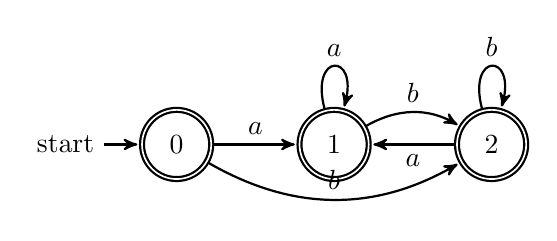
\begin{tikzpicture}[->,>=stealth',shorten >=1pt,auto,node distance=2cm,
                    thick,base node/.style={circle,draw,minimum size=16pt}, real node/.style={double,circle,draw,minimum size=35pt}]
                    \node[initial,initial text={start}, state, accepting] (1) {$0$};
                    \node[state, accepting](2)[right of=1 ]{$1$};
                    \node[state, accepting](3)[right of=2 ]{$2$};
                    \path[]
                    (1) edge node {$a$} (2)
                    (1) edge [bend right] node {$b$} (3)
                    (2) edge [loop above] node {$a$} (2)
                    (2) edge [bend left] node {$b$} (3)
                    (3) edge [loop above] node {$b$} (3)
                    (3) edge  node {$a$} (2);
                \end{tikzpicture}
            \subsubsection{DFA}
                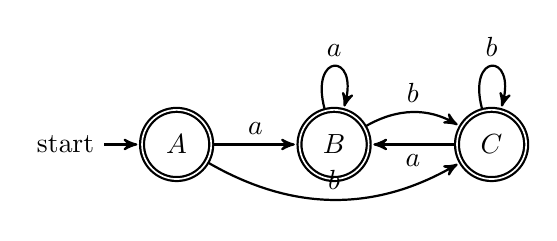
\begin{tikzpicture}[->,>=stealth',shorten >=1pt,auto,node distance=2cm,
                    thick,base node/.style={circle,draw,minimum size=16pt}, real node/.style={double,circle,draw,minimum size=35pt}]
                    \node[initial,initial text={start}, state, accepting] (1) {$A$};
                    \node[state, accepting](2)[right of=1 ]{$B$};
                    \node[state, accepting](3)[right of=2 ]{$C$};
                    \path[]
                    (1) edge node {$a$} (2)
                    (1) edge [bend right] node {$b$} (3)
                    (2) edge [loop above] node {$a$} (2)
                    (2) edge [bend left] node {$b$} (3)
                    (3) edge [loop above] node {$b$} (3)
                    (3) edge node {$a$} (2);
            \end{tikzpicture}
        \subsection{L((a|b)*a(a|b)(a|b)) [10 points]}
            \subsubsection{NFA}
                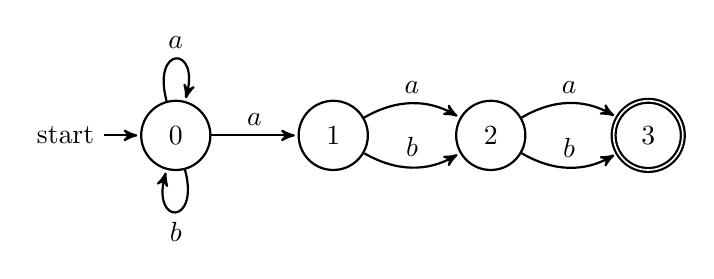
\begin{tikzpicture}[->,>=stealth',shorten >=1pt,auto,node distance=2cm,
                    thick,base node/.style={circle,draw,minimum size=16pt}, real node/.style={double,circle,draw,minimum size=35pt}]
                    \node[initial,initial text={start}, state] (1) {$0$};
                    \node[state] (2) [right of=1] {$1$};
                    \node[state] (3) [right of=2] {$2$};
                    \node[state, accepting] (4) [right of=3] {$3$};
                    \path[]
                    (1) edge [loop above] node {$a$} (1)
                    (1) edge [loop below] node {$b$} (1)
                    (1) edge node {$a$} (2)
                    (2) edge [bend left]node {$a$} (3)
                    (2) edge [bend right]node {$b$} (3)
                    (3) edge [bend left]node {$a$} (4)
                    (3) edge [bend right]node {$b$} (4);
                \end{tikzpicture}
            \subsubsection{DFA}
                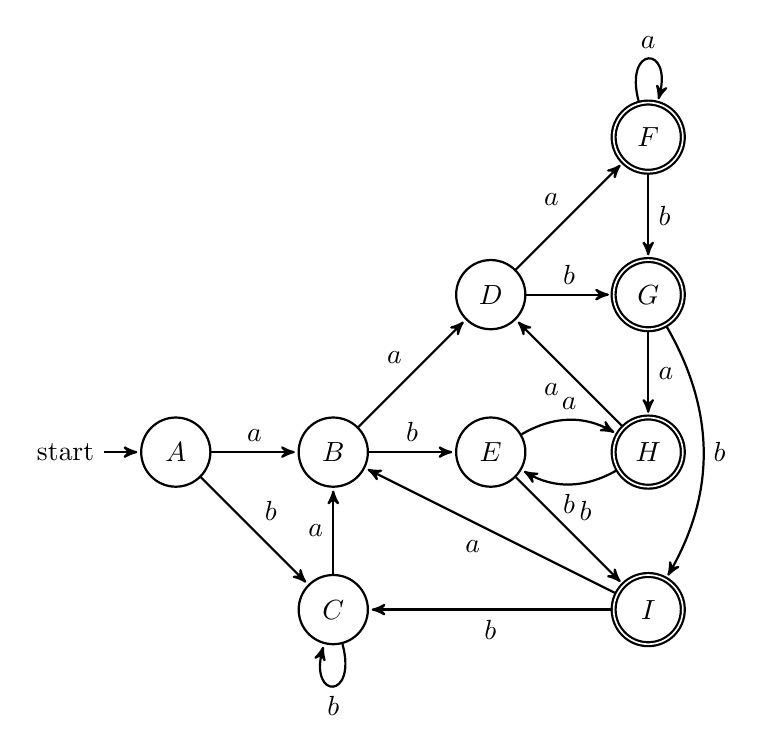
\begin{tikzpicture}[->,>=stealth',shorten >=1pt,auto,node distance=2cm,
                    thick,base node/.style={circle,draw,minimum size=16pt}, real node/.style={double,circle,draw,minimum size=35pt}]
                    \node[initial,initial text={start}, state] (1) {$A$};
                    \node[state] (2) [right of=1] {$B$};
                    \node[state] (3) [below of=2] {$C$};
                    \node[state] (5) [right of=2] {$E$};
                    \node[state] (4) [above of=5] {$D$};
                    \node[state, accepting] (7) [right of=4] {$G$};
                    \node[state, accepting] (6) [above of=7] {$F$};
                    \node[state, accepting] (8) [below of=7] {$H$};
                    \node[state, accepting] (9) [below of=8] {$I$};
                    \path[]
                    (1) edge node {$a$} (2)
                    (1) edge node {$b$} (3)
                    (2) edge node {$a$} (4)
                    (2) edge node {$b$} (5)
                    (3) edge node {$a$} (2)
                    (3) edge [loop below] node {$b$}(3)
                    (4) edge node {$a$} (6)
                    (4) edge node {$b$} (7)
                    (5) edge [bend left] node {$a$} (8)
                    (5) edge node {$b$} (9)
                    (6) edge [loop above] node {$a$} (6)
                    (6) edge node {$b$} (7)
                    (7) edge node {$a$} (8)
                    (7) edge [bend left]node {$b$} (9)
                    (8) edge node {$a$} (4)
                    (8) edge [bend left] node {$b$} (5)
                    (9) edge node {$a$} (2)
                    (9) edge node {$b$} (3)
                    ;
                \end{tikzpicture}
    \section{Exercise 2: Convert the following regular expressions to NFAs using the Thompson’s Construction Algorithm (Algorithm 3.23 in the dragon book).}
        \subsection{ (($\epsilon$|a)*b*)* [10 points]}
            \begin{itemize}
                \item Use the Basis Rule 1:
                
                    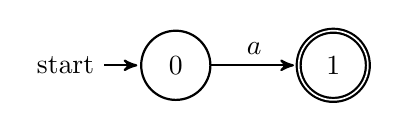
\begin{tikzpicture}[->,>=stealth',shorten >=1pt,auto,node distance=2cm,
                        thick,base node/.style={circle,draw,minimum size=16pt}, real node/.style={double,circle,draw,minimum size=35pt}]
                        \node[initial,initial text={start}, state] (1) {$0$};
                        \node[state, accepting](2)[right of=1]{$1$};
                        \path[]
                        (1) edge node {$a$} (2);
                    \end{tikzpicture}

                    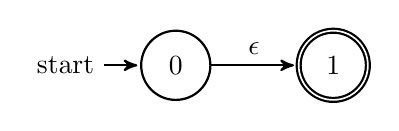
\begin{tikzpicture}[->,>=stealth',shorten >=1pt,auto,node distance=2cm,
                        thick,base node/.style={circle,draw,minimum size=16pt}, real node/.style={double,circle,draw,minimum size=35pt}]
                        \node[initial,initial text={start}, state] (1) {$0$};
                        \node[state, accepting](2)[right of=1]{$1$};
                        \path[]
                        (1) edge node {$\epsilon$} (2);
                    \end{tikzpicture}
                \item Use the Inductive Rule for the union case:
                    
                    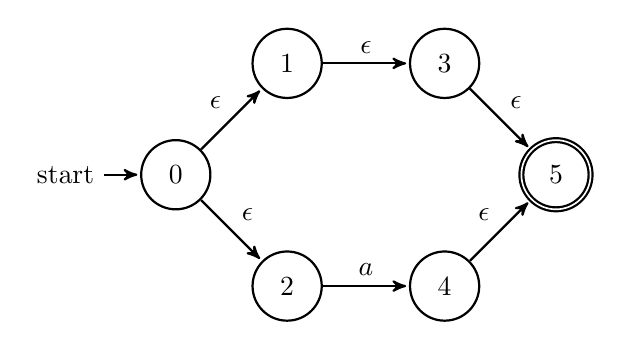
\begin{tikzpicture}[->,>=stealth',shorten >=1pt,auto,node distance=2cm,
                        thick,base node/.style={circle,draw,minimum size=16pt}, real node/.style={double,circle,draw,minimum size=35pt}]
                        \node[initial,initial text={start}, state] (1) {$0$};
                        \node[state] (2) [above right of=1] {$1$};
                        \node[state] (3) [below right of=1] {$2$};
                        \node[state] (4) [right of=2] {$3$};
                        \node[state] (5) [right of=3] {$4$};
                        \node[state, accepting] (6) [below right of=4] {$5$};
                        \path[]
                        (1) edge node {$\epsilon$} (2)
                        (1) edge node {$\epsilon$} (3)
                        (2) edge node {$\epsilon$} (4)
                        (3) edge node {$a$} (5)
                        (4) edge node {$\epsilon$} (6)
                        (5) edge node {$\epsilon$} (6);
                    \end{tikzpicture}
                \item Use the Inductive Rule for the kleene star case:
                
                    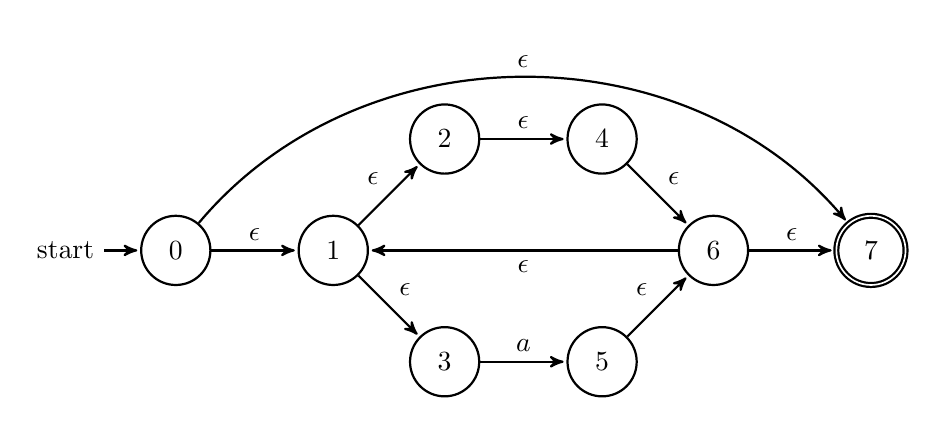
\begin{tikzpicture}[->,>=stealth',shorten >=1pt,auto,node distance=2cm,
                        thick,base node/.style={circle,draw,minimum size=16pt}, real node/.style={double,circle,draw,minimum size=35pt}]
                        \node[initial,initial text={start}, state] (0) {$0$};
                        \node[state] (1) [right of=0] {$1$};
                        \node[state] (2) [above right of=1] {$2$};
                        \node[state] (3) [below right of=1] {$3$};
                        \node[state] (4) [right of=2] {$4$};
                        \node[state] (5) [right of=3] {$5$};
                        \node[state] (6) [below right of=4] {$6$};
                        \node[state, accepting] (7) [right of=6] {$7$};
                        \path[]
                        (0) edge node {$\epsilon$} (1)
                        (1) edge node {$\epsilon$} (2)
                        (1) edge node {$\epsilon$} (3)
                        (2) edge node {$\epsilon$} (4)
                        (3) edge node {$a$} (5)
                        (4) edge node {$\epsilon$} (6)
                        (5) edge node {$\epsilon$} (6)
                        (6) edge node {$\epsilon$} (7)
                        (0) edge [bend left = 50] node {$\epsilon$} (7)
                        (6) edge node {$\epsilon$} (1);
                    \end{tikzpicture}

                    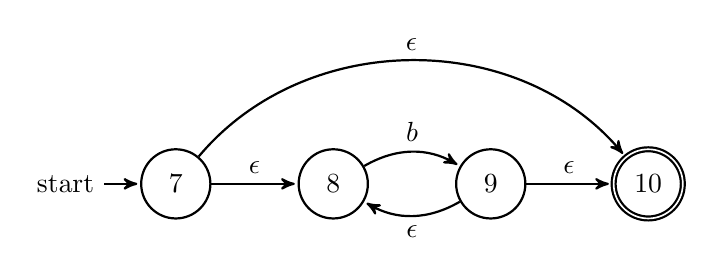
\begin{tikzpicture}[->,>=stealth',shorten >=1pt,auto,node distance=2cm,
                        thick,base node/.style={circle,draw,minimum size=16pt}, real node/.style={double,circle,draw,minimum size=35pt}]
                        \node[initial,initial text={start}, state] (7) {$7$};
                        \node[state] (8) [right of=7] {$8$};
                        \node[state] (9) [right of=8] {$9$};
                        \node[state, accepting] (10) [right of=9] {$10$};
                        \path[]
                        (7) edge node {$\epsilon$} (8)
                        (8) edge[bend left] node {$b$} (9)
                        (9) edge node {$\epsilon$} (10)
                        (7) edge[bend left = 50] node {$\epsilon$} (10)
                        (9) edge[bend left] node {$\epsilon$} (8);
                    \end{tikzpicture}
                \item Use the Inductive Rule for the concatenation case:
                
                    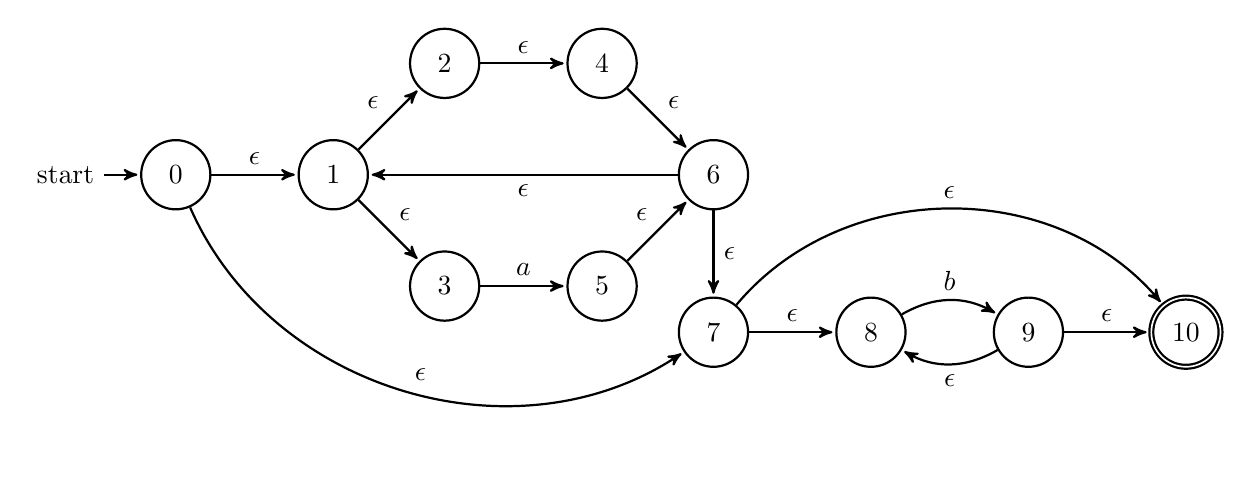
\begin{tikzpicture}[->,>=stealth',shorten >=1pt,auto,node distance=2cm,
                        thick,base node/.style={circle,draw,minimum size=16pt}, real node/.style={double,circle,draw,minimum size=35pt}]
                        \node[initial,initial text={start}, state] (0) {$0$};
                        \node[state] (1) [right of=0] {$1$};
                        \node[state] (2) [above right of=1] {$2$};
                        \node[state] (3) [below right of=1] {$3$};
                        \node[state] (4) [right of=2] {$4$};
                        \node[state] (5) [right of=3] {$5$};
                        \node[state] (6) [below right of=4] {$6$};
                        \node[state] (7) [below of=6] {$7$};
                        \node[state] (8) [right of=7] {$8$};
                        \node[state] (9) [right of=8] {$9$};
                        \node[state, accepting] (10) [right of=9] {$10$};
                        \path[]
                        (7) edge node {$\epsilon$} (8)
                        (8) edge[bend left] node {$b$} (9)
                        (9) edge node {$\epsilon$} (10)
                        (7) edge[bend left = 50] node {$\epsilon$} (10)
                        (9) edge[bend left] node {$\epsilon$} (8)
                        (0) edge node {$\epsilon$} (1)
                        (1) edge node {$\epsilon$} (2)
                        (1) edge node {$\epsilon$} (3)
                        (2) edge node {$\epsilon$} (4)
                        (3) edge node {$a$} (5)
                        (4) edge node {$\epsilon$} (6)
                        (5) edge node {$\epsilon$} (6)
                        (6) edge node {$\epsilon$} (7)
                        (0) edge [bend right = 50] node {$\epsilon$} (7)
                        (6) edge node {$\epsilon$} (1);
                    \end{tikzpicture}
                \item Use the Inductive Rule for kleene start case
                    
                    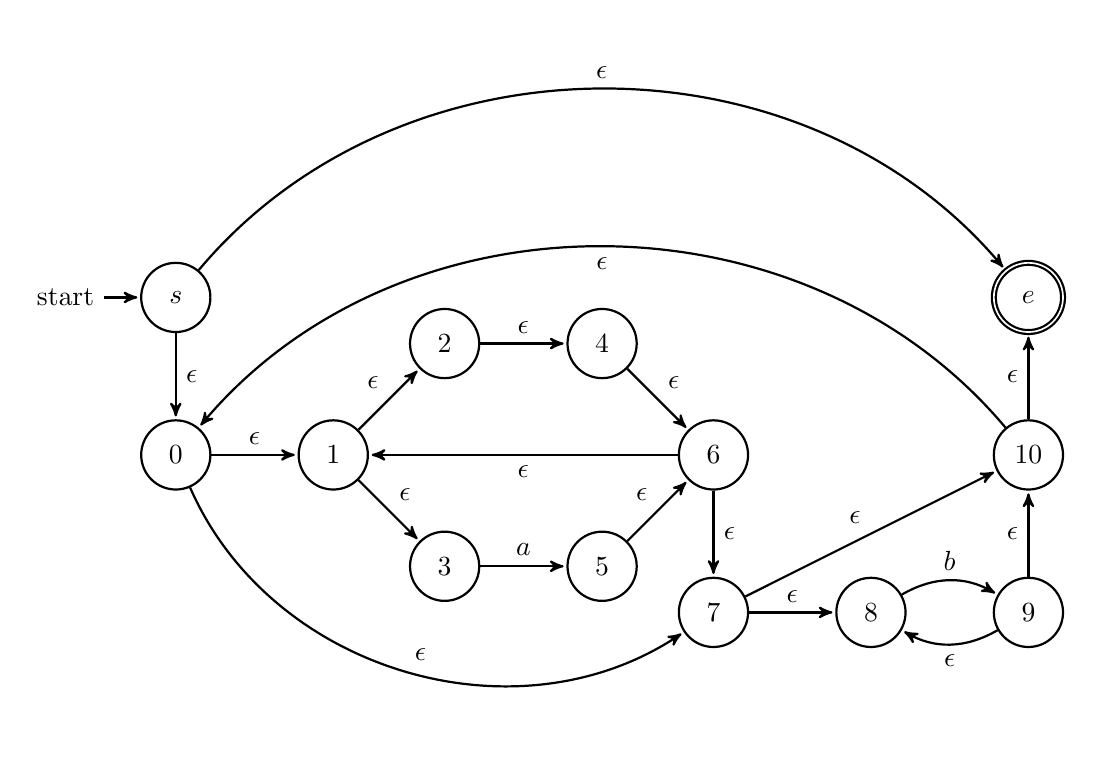
\begin{tikzpicture}[->,>=stealth',shorten >=1pt,auto,node distance=2cm,
                        thick,base node/.style={circle,draw,minimum size=16pt}, real node/.style={double,circle,draw,minimum size=35pt}]
                        \node[initial,initial text={start}, state] (s) {$s$};
                        \node[state] (0) [below of=s] {$0$};
                        \node[state] (1) [right of=0] {$1$};
                        \node[state] (2) [above right of=1] {$2$};
                        \node[state] (3) [below right of=1] {$3$};
                        \node[state] (4) [right of=2] {$4$};
                        \node[state] (5) [right of=3] {$5$};
                        \node[state] (6) [below right of=4] {$6$};
                        \node[state] (7) [below of=6] {$7$};
                        \node[state] (8) [right of=7] {$8$};
                        \node[state] (9) [right of=8] {$9$};
                        \node[state] (10) [above of=9] {$10$};
                        \node[state, accepting] (e) [above of=10] {$e$};
                        \path[]
                        (7) edge node {$\epsilon$} (8)
                        (8) edge[bend left] node {$b$} (9)
                        (9) edge node {$\epsilon$} (10)
                        (7) edge node {$\epsilon$} (10)
                        (9) edge[bend left] node {$\epsilon$} (8)
                        (0) edge node {$\epsilon$} (1)
                        (1) edge node {$\epsilon$} (2)
                        (1) edge node {$\epsilon$} (3)
                        (2) edge node {$\epsilon$} (4)
                        (3) edge node {$a$} (5)
                        (4) edge node {$\epsilon$} (6)
                        (5) edge node {$\epsilon$} (6)
                        (6) edge node {$\epsilon$} (7)
                        (0) edge [bend right = 50] node {$\epsilon$} (7)
                        (6) edge node {$\epsilon$} (1)
                        (s) edge [bend left = 50] node {$\epsilon$} (e)
                        (10) edge [bend right = 50] node {$\epsilon$} (0)
                        (s) edge node {$\epsilon$} (0)
                        (10) edge node {$\epsilon$} (e);
                    \end{tikzpicture}
            \end{itemize}
        \subsection{(a|b)*a(a|b)(a|b)[10 points]}
            \begin{itemize}
                \item Use the Basis Rule 1:
                
                    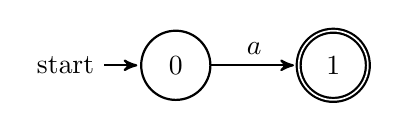
\begin{tikzpicture}[->,>=stealth',shorten >=1pt,auto,node distance=2cm,
                        thick,base node/.style={circle,draw,minimum size=16pt}, real node/.style={double,circle,draw,minimum size=35pt}]
                        \node[initial,initial text={start}, state] (1) {$0$};
                        \node[state, accepting](2)[right of=1]{$1$};
                        \path[]
                        (1) edge node {$a$} (2);
                    \end{tikzpicture}

                    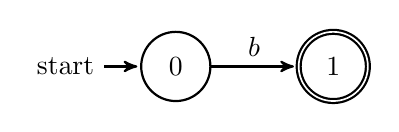
\begin{tikzpicture}[->,>=stealth',shorten >=1pt,auto,node distance=2cm,
                        thick,base node/.style={circle,draw,minimum size=16pt}, real node/.style={double,circle,draw,minimum size=35pt}]
                        \node[initial,initial text={start}, state] (1) {$0$};
                        \node[state, accepting](2)[right of=1]{$1$};
                        \path[]
                        (1) edge node {$b$} (2);
                    \end{tikzpicture}
                \item Use the Inductive Rule for the union case:
                    
                    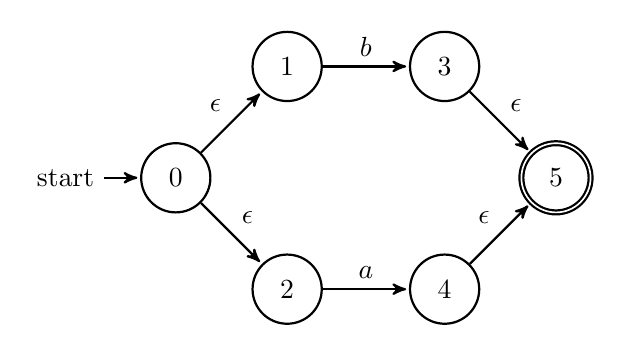
\begin{tikzpicture}[->,>=stealth',shorten >=1pt,auto,node distance=2cm,
                        thick,base node/.style={circle,draw,minimum size=16pt}, real node/.style={double,circle,draw,minimum size=35pt}]
                        \node[initial,initial text={start}, state] (1) {$0$};
                        \node[state] (2) [above right of=1] {$1$};
                        \node[state] (3) [below right of=1] {$2$};
                        \node[state] (4) [right of=2] {$3$};
                        \node[state] (5) [right of=3] {$4$};
                        \node[state, accepting] (6) [below right of=4] {$5$};
                        \path[]
                        (1) edge node {$\epsilon$} (2)
                        (1) edge node {$\epsilon$} (3)
                        (2) edge node {$b$} (4)
                        (3) edge node {$a$} (5)
                        (4) edge node {$\epsilon$} (6)
                        (5) edge node {$\epsilon$} (6);
                    \end{tikzpicture}
                \item Use the Inductive Rule for the kleene star case:
            
                    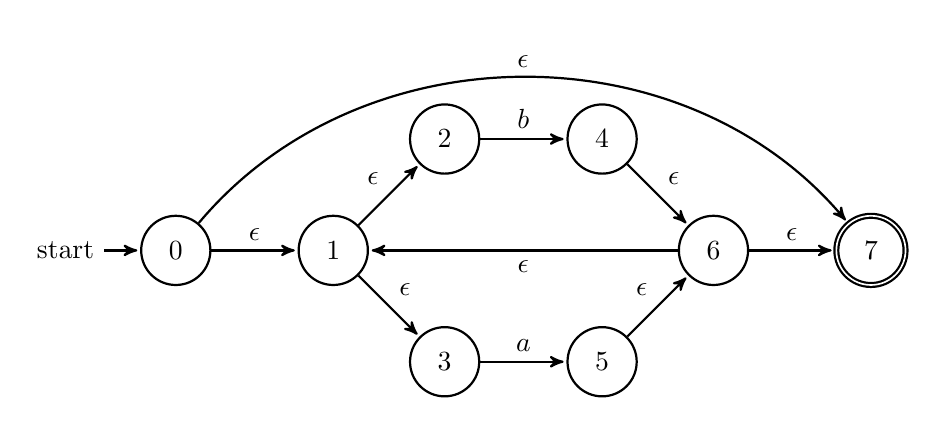
\begin{tikzpicture}[->,>=stealth',shorten >=1pt,auto,node distance=2cm,
                        thick,base node/.style={circle,draw,minimum size=16pt}, real node/.style={double,circle,draw,minimum size=35pt}]
                        \node[initial,initial text={start}, state] (0) {$0$};
                        \node[state] (1) [right of=0] {$1$};
                        \node[state] (2) [above right of=1] {$2$};
                        \node[state] (3) [below right of=1] {$3$};
                        \node[state] (4) [right of=2] {$4$};
                        \node[state] (5) [right of=3] {$5$};
                        \node[state] (6) [below right of=4] {$6$};
                        \node[state, accepting] (7) [right of=6] {$7$};
                        \path[]
                        (0) edge node {$\epsilon$} (1)
                        (1) edge node {$\epsilon$} (2)
                        (1) edge node {$\epsilon$} (3)
                        (2) edge node {$b$} (4)
                        (3) edge node {$a$} (5)
                        (4) edge node {$\epsilon$} (6)
                        (5) edge node {$\epsilon$} (6)
                        (6) edge node {$\epsilon$} (7)
                        (0) edge [bend left = 50] node {$\epsilon$} (7)
                        (6) edge node {$\epsilon$} (1);
                    \end{tikzpicture}
                \item Use the Inductive Rule for the concatenation case:
                
                    \begin{tikzpicture}[->,>=stealth',shorten >=1pt,auto,node distance=2cm,
                        thick,base node/.style={circle,draw,minimum size=16pt}, real node/.style={double,circle,draw,minimum size=35pt}]
                        \node[initial,initial text={start}, state] (s) {$s$};
                        \node[state] (1) [right of=s] {$1$};
                        \node[state] (2) [above right of=1] {$2$};
                        \node[state] (3) [below right of=1] {$3$};
                        \node[state] (4) [right of=2] {$4$};
                        \node[state] (5) [right of=3] {$5$};
                        \node[state] (6) [below right of=4] {$6$};
                        \node[state] (7) [below of=6] {$7$};
                        \node[state] (8) [right of=7] {$8$};
                        \node[state] (9) [below right of=8] {$9$};
                        \node[state] (10)[below of = 9] {$10$};
                        \node[state] (11)[above left of = 10] {$11$};
                        \node[state] (12)[below left of = 10] {$12$};
                        \node[state] (13)[left of = 11] {$13$};
                        \node[state] (14)[left of = 12] {$14$};
                        \node[state] (15)[below left of = 13] {$15$};
                        \node[state] (16)[left of = 15] {$16$};
                        \node[state] (17)[above left of = 16] {$17$};
                        \node[state] (18)[below left of = 16] {$18$};
                        \node[state] (19)[left of = 17] {$19$};
                        \node[state] (20)[left of = 18] {$20$};
                        \node[state, accepting] (e) [below left of=19] {$e$};
                        \path[]
                        (s) edge node {$\epsilon$} (1)
                        (1) edge node {$\epsilon$} (2)
                        (1) edge node {$\epsilon$} (3)
                        (2) edge node {$b$} (4)
                        (3) edge node {$a$} (5)
                        (4) edge node {$\epsilon$} (6)
                        (5) edge node {$\epsilon$} (6)
                        (6) edge node {$\epsilon$} (7)
                        (0) edge [bend right = 50] node {$\epsilon$} (7)
                        (6) edge node {$\epsilon$} (1)
                        (7) edge node {$a$} (8)
                        (8) edge node {$\epsilon$} (9)
                        (9) edge node {$\epsilon$} (10)
                        (10) edge node {$\epsilon$} (11)
                        (10) edge node {$\epsilon$} (12)
                        (11) edge node {$a$} (13)
                        (12) edge node {$b$} (14)
                        (13) edge node {$\epsilon$} (15)
                        (14) edge node {$\epsilon$} (15)
                        (15) edge node {$\epsilon$} (16)
                        (16) edge node {$\epsilon$} (17)
                        (16) edge node {$\epsilon$} (18)
                        (17) edge node {$a$} (19)
                        (18) edge node {$b$} (20)
                        (19) edge node {$\epsilon$} (e)
                        (20) edge node {$\epsilon$} (e);
                    \end{tikzpicture}
            \end{itemize}
        \subsection{a*ba*ba*ba* [10 points]}
            \begin{itemize}
                \item Use the Inductive Rule for the kleene star case:

                    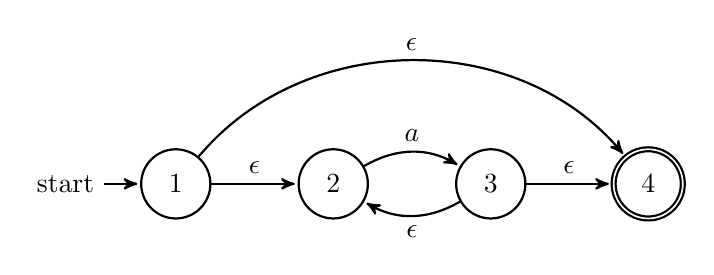
\begin{tikzpicture}[->,>=stealth',shorten >=1pt,auto,node distance=2cm,
                        thick,base node/.style={circle,draw,minimum size=16pt}, real node/.style={double,circle,draw,minimum size=35pt}]
                        \node[initial,initial text={start}, state] (1) {$1$};
                        \node[state] (2) [right of=1] {$2$};
                        \node[state] (3) [right of=2] {$3$};
                        \node[state, accepting] (4) [right of=3] {$4$};
                        \path[]
                        (1) edge node {$\epsilon$} (2)
                        (2) edge[bend left] node {$a$} (3)
                        (3) edge node {$\epsilon$} (4)
                        (1) edge[bend left = 50] node {$\epsilon$} (4)
                        (3) edge[bend left] node {$\epsilon$} (2);
                    \end{tikzpicture}
                \item Use the Inductive Rule for the concatenation case:
                    
                    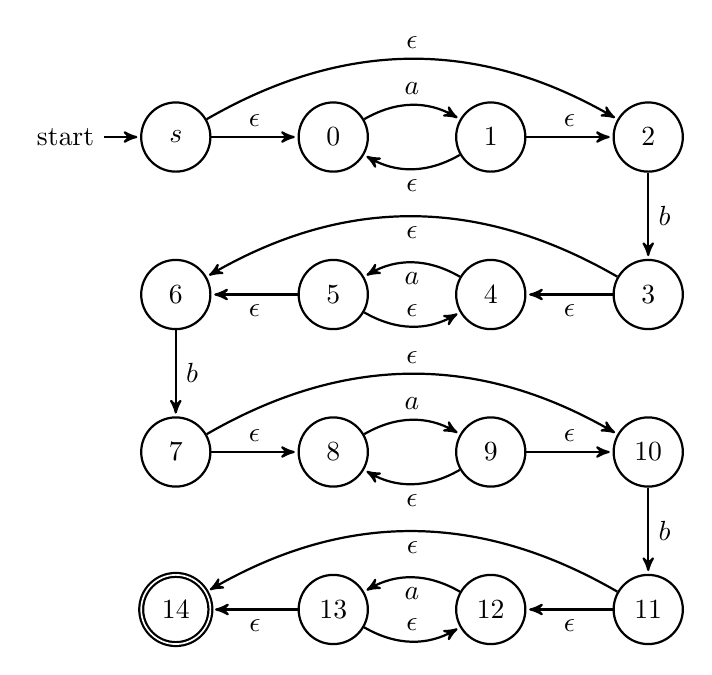
\begin{tikzpicture}[->,>=stealth',shorten >=1pt,auto,node distance=2cm,
                        thick,base node/.style={circle,draw,minimum size=16pt}, real node/.style={double,circle,draw,minimum size=35pt}]
                        \node[initial,initial text={start}, state] (s) {$s$};
                        \node[state] (0) [right of=s] {$0$};
                        \node[state] (1) [right of=0] {$1$};
                        \node[state] (2) [right of=1] {$2$};

                        \node[state] (3) [below of=2] {$3$};
                        \node[state] (4) [left of=3] {$4$};
                        \node[state] (5) [left of=4] {$5$};
                        \node[state] (6) [left of=5] {$6$};

                        \node[state] (7) [below of=6] {$7$};
                        \node[state] (8) [right of=7] {$8$};
                        \node[state] (9) [right of=8] {$9$};
                        \node[state] (10) [right of=9] {$10$};

                        \node[state] (11) [below of=10] {$11$};
                        \node[state] (12) [left of=11] {$12$};
                        \node[state] (13) [left of=12] {$13$};
                        \node[state, accepting] (14) [left of=13] {$14$};
                        \path[]
                        (s) edge node {$\epsilon$} (0)
                        (s) edge[bend left = 30] node {$\epsilon$} (2)
                        (0) edge[bend left] node {$a$} (1)
                        (1) edge[bend left] node {$\epsilon$} (0)
                        (1) edge node {$\epsilon$} (2)
                        
                        (2) edge node {$b$} (3)

                        (3) edge node {$\epsilon$} (4)
                        (3) edge[bend right = 30] node {$\epsilon$} (6)
                        (4) edge[bend right] node {$a$} (5)
                        (5) edge[bend right] node {$\epsilon$} (4)
                        (5) edge node {$\epsilon$} (6)

                        (6) edge node {$b$} (7)

                        (7) edge node {$\epsilon$} (8)
                        (7) edge[bend left = 30] node {$\epsilon$} (10)
                        (8) edge[bend left] node {$a$} (9)
                        (9) edge[bend left] node {$\epsilon$} (8)
                        (9) edge node {$\epsilon$} (10)

                        (10) edge node {$b$} (11)

                        (11) edge node {$\epsilon$} (12)
                        (11) edge[bend right = 30] node {$\epsilon$} (14)
                        (12) edge[bend right] node {$a$} (13)
                        (13) edge[bend right] node {$\epsilon$} (12)
                        (13) edge node {$\epsilon$} (14)
                        ;
                    \end{tikzpicture}
            \end{itemize}
    \section{Exercise 3: Convert the NFAs in Exercise 2 to DFAs using the Subset Construction Algorithm (Algorithm 3.20 in the dragon book). [30 points in total; 10 points for each correct conversion]}
        \subsection{(($\epsilon$|a)* b*)* [10 points]}
            
            NFA is :

            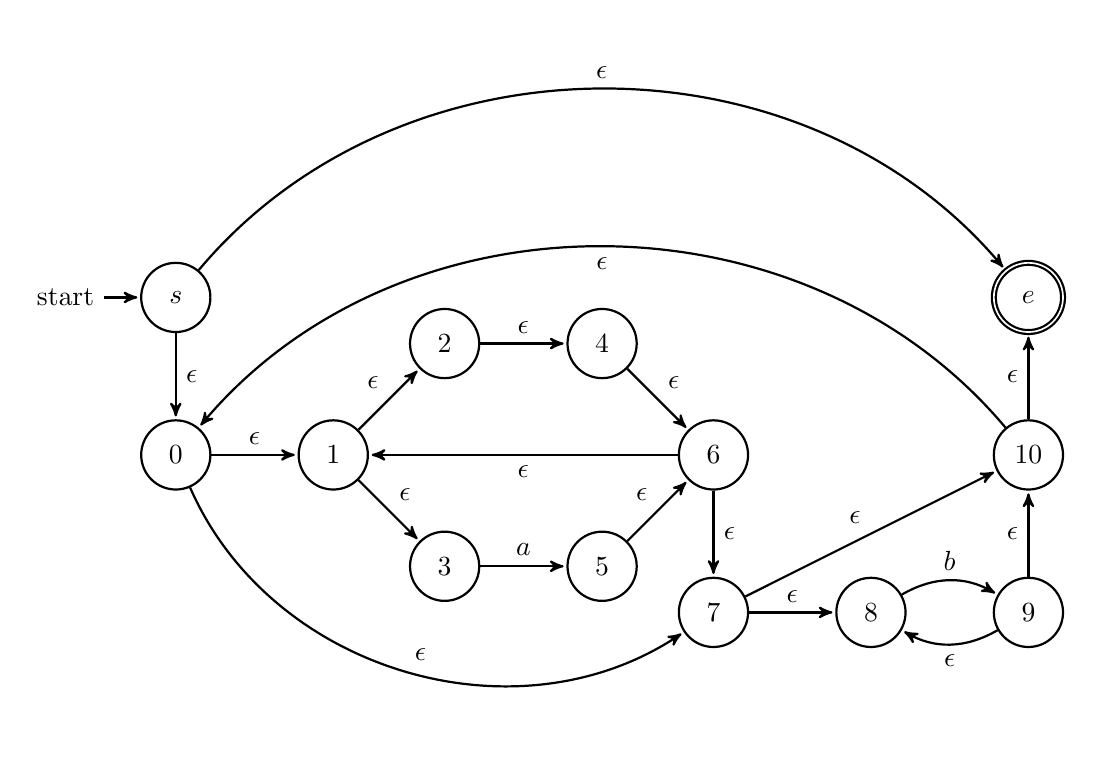
\begin{tikzpicture}[->,>=stealth',shorten >=1pt,auto,node distance=2cm,
                thick,base node/.style={circle,draw,minimum size=16pt}, real node/.style={double,circle,draw,minimum size=35pt}]
                \node[initial,initial text={start}, state] (s) {$s$};
                \node[state] (0) [below of=s] {$0$};
                \node[state] (1) [right of=0] {$1$};
                \node[state] (2) [above right of=1] {$2$};
                \node[state] (3) [below right of=1] {$3$};
                \node[state] (4) [right of=2] {$4$};
                \node[state] (5) [right of=3] {$5$};
                \node[state] (6) [below right of=4] {$6$};
                \node[state] (7) [below of=6] {$7$};
                \node[state] (8) [right of=7] {$8$};
                \node[state] (9) [right of=8] {$9$};
                \node[state] (10) [above of=9] {$10$};
                \node[state, accepting] (e) [above of=10] {$e$};
                \path[]
                (7) edge node {$\epsilon$} (8)
                (8) edge[bend left] node {$b$} (9)
                (9) edge node {$\epsilon$} (10)
                (7) edge node {$\epsilon$} (10)
                (9) edge[bend left] node {$\epsilon$} (8)
                (0) edge node {$\epsilon$} (1)
                (1) edge node {$\epsilon$} (2)
                (1) edge node {$\epsilon$} (3)
                (2) edge node {$\epsilon$} (4)
                (3) edge node {$a$} (5)
                (4) edge node {$\epsilon$} (6)
                (5) edge node {$\epsilon$} (6)
                (6) edge node {$\epsilon$} (7)
                (0) edge [bend right = 50] node {$\epsilon$} (7)
                (6) edge node {$\epsilon$} (1)
                (s) edge [bend left = 50] node {$\epsilon$} (e)
                (10) edge [bend right = 50] node {$\epsilon$} (0)
                (s) edge node {$\epsilon$} (0)
                (10) edge node {$\epsilon$} (e);
            \end{tikzpicture}

            If use the subset construction algorithm:
                \begin{enumerate}[\qquad 1. ]
                    \item Q1 = \{s,0,1,2,3,4,6,7,8,10,e\}
                    \item Q2 = \{0,1,2,3,4,5,6,7,8,10,e\}
                    \item Q3 = \{0,1,2,3,4,6,7,8,9,10,e\}
                \end{enumerate}

            DFA status transfer table:
                
                \begin{table}[!htbp]
                    \centering
                    \caption{(($\epsilon$|a)* b*)*}
                    \label{tab:aStrangeTable}
                    \begin{tabular}{ccc}
                        \hline
                        DFA Status  & a     & b     \\
                        \hline
                        Q1          & Q2    & Q3    \\
                        \hline
                        Q2          & Q2    & Q3    \\
                        \hline
                        Q3          & Q2    & Q3    \\
                        \hline
                    \end{tabular}
                \end{table}

            DFA

                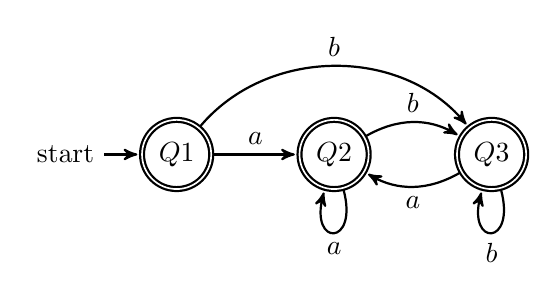
\begin{tikzpicture}[->,>=stealth',shorten >=1pt,auto,node distance=2cm,
                    thick,base node/.style={circle,draw,minimum size=16pt}, real node/.style={double,circle,draw,minimum size=35pt}]
                    \node[initial,initial text={start}, state, accepting] (0) {$Q1$};
                    \node[state, accepting] (1) [right of=0] {$Q2$};
                    \node[state, accepting] (2) [right of=1] {$Q3$};
                    \path[]
                    (0) edge node {$a$} (1)
                    (0) edge [bend left = 50] node {$b$} (2)
                    (1) edge [loop below] node {$a$} (1)
                    (1) edge [bend left = 30] node {$b$} (2)
                    (2) edge [bend left = 30] node {$a$} (1)
                    (2) edge [loop below] node {$b$} (2)
                    ;
                \end{tikzpicture}
        \subsection{(a|b)*a(a|b)(a|b)[10 points]}

            NFA is:

            \begin{tikzpicture}[->,>=stealth',shorten >=1pt,auto,node distance=2cm,
                thick,base node/.style={circle,draw,minimum size=16pt}, real node/.style={double,circle,draw,minimum size=35pt}]
                \node[initial,initial text={start}, state] (s) {$s$};
                \node[state] (1) [right of=s] {$1$};
                \node[state] (2) [above right of=1] {$2$};
                \node[state] (3) [below right of=1] {$3$};
                \node[state] (4) [right of=2] {$4$};
                \node[state] (5) [right of=3] {$5$};
                \node[state] (6) [below right of=4] {$6$};
                \node[state] (7) [below of=6] {$7$};
                \node[state] (8) [right of=7] {$8$};
                \node[state] (9) [below right of=8] {$9$};
                \node[state] (10)[below of = 9] {$10$};
                \node[state] (11)[above left of = 10] {$11$};
                \node[state] (12)[below left of = 10] {$12$};
                \node[state] (13)[left of = 11] {$13$};
                \node[state] (14)[left of = 12] {$14$};
                \node[state] (15)[below left of = 13] {$15$};
                \node[state] (16)[left of = 15] {$16$};
                \node[state] (17)[above left of = 16] {$17$};
                \node[state] (18)[below left of = 16] {$18$};
                \node[state] (19)[left of = 17] {$19$};
                \node[state] (20)[left of = 18] {$20$};
                \node[state, accepting] (e) [below left of=19] {$e$};
                \path[]
                (s) edge node {$\epsilon$} (1)
                (1) edge node {$\epsilon$} (2)
                (1) edge node {$\epsilon$} (3)
                (2) edge node {$b$} (4)
                (3) edge node {$a$} (5)
                (4) edge node {$\epsilon$} (6)
                (5) edge node {$\epsilon$} (6)
                (6) edge node {$\epsilon$} (7)
                (0) edge [bend right = 50] node {$\epsilon$} (7)
                (6) edge node {$\epsilon$} (1)
                (7) edge node {$a$} (8)
                (8) edge node {$\epsilon$} (9)
                (9) edge node {$\epsilon$} (10)
                (10) edge node {$\epsilon$} (11)
                (10) edge node {$\epsilon$} (12)
                (11) edge node {$a$} (13)
                (12) edge node {$b$} (14)
                (13) edge node {$\epsilon$} (15)
                (14) edge node {$\epsilon$} (15)
                (15) edge node {$\epsilon$} (16)
                (16) edge node {$\epsilon$} (17)
                (16) edge node {$\epsilon$} (18)
                (17) edge node {$a$} (19)
                (18) edge node {$b$} (20)
                (19) edge node {$\epsilon$} (e)
                (20) edge node {$\epsilon$} (e);
            \end{tikzpicture}

            If use the subset construction algorithm:
            \begin{enumerate}[\qquad 1. ]
                \item Q1 = \{s,1,2,3,7\}
                \item Q2 = \{1,2,3,5,6,7,8,9,10,11,12\}
                \item Q3 = \{1,2,3,4,6,7\}
                \item Q4 = Q2+\{13,15,16,17,18\}
                \item Q5 = Q3+\{14,15,16,17,18\}
                \item Q6 = Q4+\{19,e\}
                \item Q7 = Q5+\{20,e\}
                \item Q8 = Q2+\{19,e\}
                \item Q9 = Q3+\{20,e\}
            \end{enumerate}

            DFA status transfer table:
                
                \begin{table}[!htbp]
                    \centering
                    \caption{(a|b)*a(a|b)(a|b)[10 points]}
                    \label{tab:aStrangeTable}
                    \begin{tabular}{ccc}
                        \hline
                        DFA Status  & a     & b     \\
                        \hline
                        Q1          & Q2    & Q3    \\
                        \hline
                        Q2          & Q4    & Q5    \\
                        \hline
                        Q3          & Q2    & Q3    \\
                        \hline
                        Q4          & Q6    & Q7    \\
                        \hline
                        Q5          & Q8    & Q9    \\
                        \hline
                        Q6          & Q6    & Q7    \\
                        \hline
                        Q7          & Q8    & Q9    \\
                        \hline
                        Q8          & Q4    & Q5    \\
                        \hline
                        Q9          & Q2    & Q3    \\    
                        \hline

                    \end{tabular}
                \end{table}
            
            DFA is:

                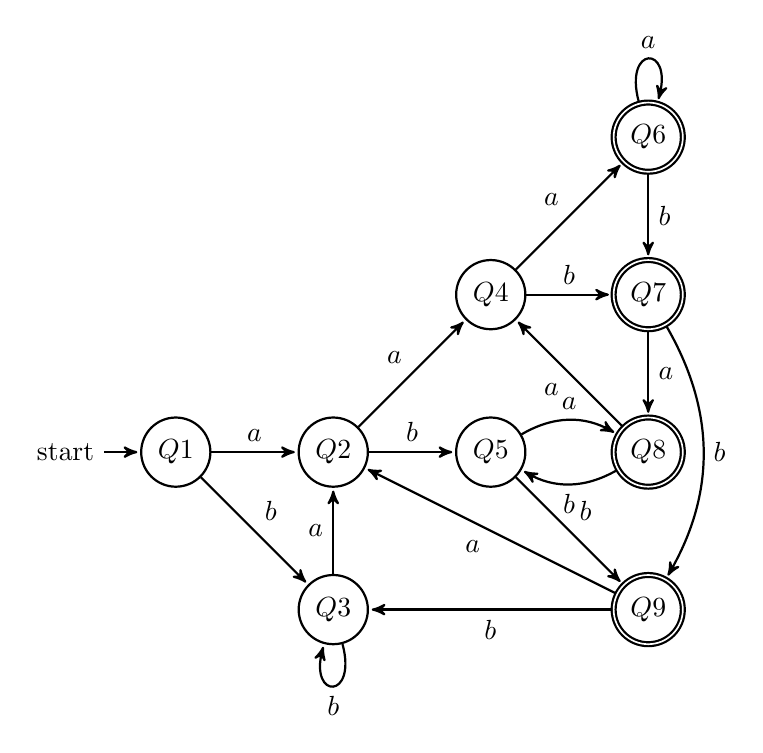
\begin{tikzpicture}[->,>=stealth',shorten >=1pt,auto,node distance=2cm,
                    thick,base node/.style={circle,draw,minimum size=16pt}, real node/.style={double,circle,draw,minimum size=35pt}]
                    \node[initial,initial text={start}, state] (1) {$Q1$};
                    \node[state] (2) [right of=1] {$Q2$};
                    \node[state] (3) [below of=2] {$Q3$};
                    \node[state] (5) [right of=2] {$Q5$};
                    \node[state] (4) [above of=5] {$Q4$};
                    \node[state, accepting] (7) [right of=4] {$Q7$};
                    \node[state, accepting] (6) [above of=7] {$Q6$};
                    \node[state, accepting] (8) [below of=7] {$Q8$};
                    \node[state, accepting] (9) [below of=8] {$Q9$};
                    \path[]
                    (1) edge node {$a$} (2)
                    (1) edge node {$b$} (3)
                    (2) edge node {$a$} (4)
                    (2) edge node {$b$} (5)
                    (3) edge node {$a$} (2)
                    (3) edge [loop below] node {$b$}(3)
                    (4) edge node {$a$} (6)
                    (4) edge node {$b$} (7)
                    (5) edge [bend left] node {$a$} (8)
                    (5) edge node {$b$} (9)
                    (6) edge [loop above] node {$a$} (6)
                    (6) edge node {$b$} (7)
                    (7) edge node {$a$} (8)
                    (7) edge [bend left]node {$b$} (9)
                    (8) edge node {$a$} (4)
                    (8) edge [bend left] node {$b$} (5)
                    (9) edge node {$a$} (2)
                    (9) edge node {$b$} (3)
                    ;
                \end{tikzpicture}
        \subsection{a*ba*ba*ba* [10 points]}
            NFA is:

            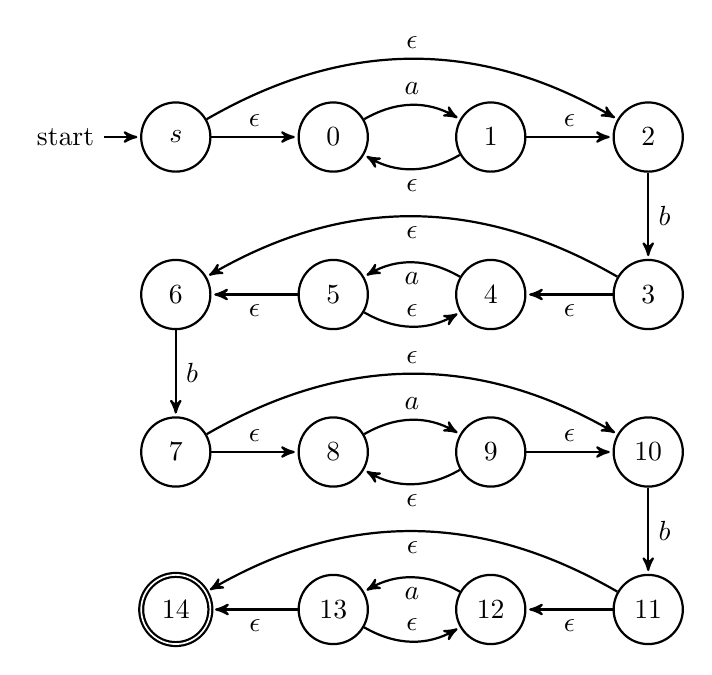
\begin{tikzpicture}[->,>=stealth',shorten >=1pt,auto,node distance=2cm,
                thick,base node/.style={circle,draw,minimum size=16pt}, real node/.style={double,circle,draw,minimum size=35pt}]
                \node[initial,initial text={start}, state] (s) {$s$};
                \node[state] (0) [right of=s] {$0$};
                \node[state] (1) [right of=0] {$1$};
                \node[state] (2) [right of=1] {$2$};

                \node[state] (3) [below of=2] {$3$};
                \node[state] (4) [left of=3] {$4$};
                \node[state] (5) [left of=4] {$5$};
                \node[state] (6) [left of=5] {$6$};

                \node[state] (7) [below of=6] {$7$};
                \node[state] (8) [right of=7] {$8$};
                \node[state] (9) [right of=8] {$9$};
                \node[state] (10) [right of=9] {$10$};

                \node[state] (11) [below of=10] {$11$};
                \node[state] (12) [left of=11] {$12$};
                \node[state] (13) [left of=12] {$13$};
                \node[state, accepting] (14) [left of=13] {$14$};
                \path[]
                (s) edge node {$\epsilon$} (0)
                (s) edge[bend left = 30] node {$\epsilon$} (2)
                (0) edge[bend left] node {$a$} (1)
                (1) edge[bend left] node {$\epsilon$} (0)
                (1) edge node {$\epsilon$} (2)
                
                (2) edge node {$b$} (3)

                (3) edge node {$\epsilon$} (4)
                (3) edge[bend right = 30] node {$\epsilon$} (6)
                (4) edge[bend right] node {$a$} (5)
                (5) edge[bend right] node {$\epsilon$} (4)
                (5) edge node {$\epsilon$} (6)

                (6) edge node {$b$} (7)

                (7) edge node {$\epsilon$} (8)
                (7) edge[bend left = 30] node {$\epsilon$} (10)
                (8) edge[bend left] node {$a$} (9)
                (9) edge[bend left] node {$\epsilon$} (8)
                (9) edge node {$\epsilon$} (10)

                (10) edge node {$b$} (11)

                (11) edge node {$\epsilon$} (12)
                (11) edge[bend right = 30] node {$\epsilon$} (14)
                (12) edge[bend right] node {$a$} (13)
                (13) edge[bend right] node {$\epsilon$} (12)
                (13) edge node {$\epsilon$} (14)
                ;
            \end{tikzpicture}

            If use the subset construction algorithm:
            \begin{enumerate}[\qquad 1. ]
                \item Q1 = \{s,0,2\}
                \item Q2 = \{0,1,2\}
                \item Q3 = \{3,4,6\}
                \item Q4 = \{4,5,6\}
                \item Q5 = \{7,8,10\}
                \item Q6 = \{8,9,10\}
                \item Q7 = \{11,12,14\}
                \item Q8 = \{12,13,14\}
            \end{enumerate}

            DFA status transfer table:
                
                \begin{table}[!htbp]
                    \centering
                    \caption{a*ba*ba*ba*}
                    \label{tab:aStrangeTable}
                    \begin{tabular}{ccc}
                        \hline
                        DFA Status  & a     & b     \\
                        \hline
                        Q1          & Q2    & Q3    \\
                        \hline
                        Q2          & Q2    & Q3    \\
                        \hline
                        Q3          & Q4    & Q5    \\
                        \hline
                        Q4          & Q4    & Q5    \\
                        \hline
                        Q5          & Q6    & Q7    \\
                        \hline
                        Q6          & Q6    & Q7    \\
                        \hline
                        Q7          & Q8    & $\epsilon$ \\
                        \hline
                        Q8          & Q8    & $\epsilon$ \\
                        \hline
                    \end{tabular}
                \end{table}

            DFA:

                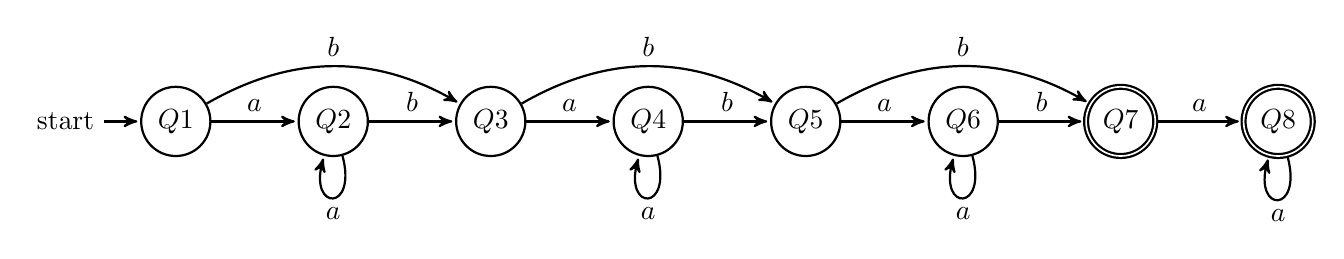
\begin{tikzpicture}[->,>=stealth',shorten >=1pt,auto,node distance=2cm,
                    thick,base node/.style={circle,draw,minimum size=16pt}, real node/.style={double,circle,draw,minimum size=35pt}]
                    \node[initial,initial text={start}, state] (1) {$Q1$};
                    \node[state] (2) [right of=1] {$Q2$};
                    \node[state] (3) [right of=2] {$Q3$};
                    \node[state] (4) [right of=3] {$Q4$};
                    \node[state] (5) [right of=4] {$Q5$};
                    \node[state] (6) [right of=5] {$Q6$};
                    \node[state, accepting] (7) [right of=6] {$Q7$};
                    \node[state, accepting] (8) [right of=7] {$Q8$};
                    \path[]
                    (1) edge node {$a$} (2)
                    (1) edge [bend left] node {$b$} (3)
                    (2) edge [loop below] node {$a$} (2)
                    (2) edge node {$b$} (3)
                    (3) edge node {$a$} (4)
                    (3) edge [bend left] node {$b$} (5)
                    (4) edge [loop below] node {$a$} (4)
                    (4) edge node {$b$} (5)
                    (5) edge node {$a$} (6)
                    (5) edge [bend left] node {$b$} (7)
                    (6) edge [loop below] node {$a$} (6)
                    (6) edge node {$b$} (7)
                    (7) edge node {$a$} (8)
                    (8) edge [loop below] node {$a$} (8)
                    ;
                \end{tikzpicture}

\end{document}